% Chapter 1

\chapter{Standard model and supersymmetry} % Main chapter title

\label{Chap1} % For referencing the chapter elsewhere, use \ref{Chapter1} 

%----------------------------------------------------------------------------------------

% Define some commands to keep the formatting separated from the content 
\newcommand{\keyword}[1]{\textbf{#1}}
\newcommand{\tabhead}[1]{\textbf{#1}}
\newcommand{\code}[1]{\texttt{#1}}
\newcommand{\file}[1]{\texttt{\bfseries#1}}
\newcommand{\option}[1]{\texttt{\itshape#1}}

\section{Standard model particles}
The SM of particle physics consists of 3 \textit{generations} of quarks and leptons (Table \ref{tab:SM}), gauge bosons which are mediators 
of strong, electromagnetic (EM) and weak force, and a scalar Higgs boson (Table \ref{tab:SM_boson}).

\begin{table}[h!]
\centering
\caption{Leptons and quarks of SM with their properties}
\label{tab:SM}
\begin{tabular}{c|c|c|c|c|c}
\hline
\multicolumn{6}{c}{Leptons (spin \textonehalf)}\\ \hline
Gen.         & Particle & Charge & Mass (MeV) & Interactions\footnotemark & Chiral state\\ \hline
%				   &		  &		   &            &               &\\ \hline
\multirow{2}{*}{1} & $\nu_e$  &  0     & $<2\times10^{-6}$     & Weak & \multirow{2}{*}{$\begin{bmatrix} \nu_e \\ e_{L}\end{bmatrix},\ e_{R}$}\\
& $e$      &	 $\mp1$ & 0.511  & EM, Weak      &	\\ \hline
\multirow{2}{*}{2} & $\nu_\mu$  &  0     & $<0.19$  & Weak & \multirow{2}{*}{$\begin{bmatrix} \nu_\mu \\ \mu_{L}\end{bmatrix},\ \mu_{R}$}\\
& $\mu$      &	 $\mp1$ & 105.7  & EM, Weak      &	\\ \hline
\multirow{2}{*}{3} & $\nu_\tau$  &  0     & $<18.2$  & Weak & \multirow{2}{*}{$\begin{bmatrix} \nu_\tau \\ \tau_{L}\end{bmatrix},\ \tau_{R}$}\\
& $\tau$      &	 $\mp1$ & 1777  & EM, Weak      &	\\ \hline

\multicolumn{6}{c}{Quarks (spin \textonehalf)}\\ \hline
Gen.        & Particle & Charge & Mass (MeV) & Interactions & Chiral state\\ \hline
\multirow{2}{*}{1} & $u$  &  $\pm\frac{2}{3}$     & $\approx 2.2$     & \multirow{6}{*}{Strong, EM, \newline Weak} & \multirow{2}{*}{$\begin{bmatrix} u_L \\ d_{L}\end{bmatrix},\ u_{R},\ d_R$}\\
 & $d$      &	 $\mp\frac{1}{3}$ & $\approx4.7$  &       &	\\ \cline{1-4} \cline{6-6}
\multirow{2}{*}{2} & $c$  &  $\pm\frac{2}{3}$     & $1.275\times10^{3}$     &  & \multirow{2}{*}{$\begin{bmatrix} c_L \\ s_{L}\end{bmatrix},\ c_{R},\ s_R$}\\
 & $s$      &	 $\mp\frac{1}{3}$ & $\approx95$  &       &	\\ \cline{1-4} \cline{6-6}
\multirow{2}{*}{3} & $t$  &  $\pm\frac{2}{3}$     & $173.1\times10^{3}$     &  & \multirow{2}{*}{$\begin{bmatrix} t_L \\ b_{L}\end{bmatrix},\ t_{R},\ b_R$}\\
 & $b$      &	 $\mp\frac{1}{3}$ & $\approx4.18\times10^{3}$  &       &	\\ \hline
\end{tabular}
\end{table}
\footnotetext{All particles with non-zero mass have gravitational interactions. But gravity is not a part of SM.}

\begin{table}[h!]
\centering
\captionsetup{width=.9\linewidth}
\caption{Gauge bosons and higgs boson in SM with their properties}
\label{tab:SM_boson}
\begin{tabular}{c|c|c|c|c|c}
\hline
Particle	&	Charge	&	Mass (GeV)	&	Spin	&	Force mediation	&	Mixing fields\\\hline
g			&	0		&	0			&	1		&	Strong			&	g\\
$\gamma$	&	0		&	0			&	1		&	EM				&	$W_3,B$\\
\ce{W}			&	$\mp1$	&	80.4		&	1		&	Weak			&	$W_1,W_2$\\
\ce{Z}			&	0		&	91.2		&	1		&	Weak			&	$W_3,B$\\
\ce{H}			&	0		&	125.2		&	0		&	-				&	$H_u,H_d$\\\hline
\end{tabular}
\end{table}
Categorization of the quarks and leptons into 3 generations is done based on their masses~\cite{PhysRevD.98.030001} and properties. The 
first generation consists of lightest and the third generation consists of heaviest particles. Neutrinos are grouped according to their 
interactions and their exact masses are unknown. The masses of SM particles are not predicted by the theory, but they are measured 
quantities in experiments. All the charged (in this thesis charge always refers to electric charge) particles can interact via EM force. 
Neutral leptons, neutrinos, are allowed to undergo only weak interactions. Quarks have an additional quantum number, color, which is responsible for strong 
interaction. 

\section{Conservation laws and symmetry}\label{sec:consvLaws}
Experiments have played a significant role in development of the SM. Various observations from them lead to framing many laws of nature. 
Similar to the law of conservation of energy, linear momentum and angular momentum in basic physics, there are other laws of conservation 
such as charge, color charge, lepton number within each generation etc. Whenever there is a conservation law, then there is a symmetry 
associated with it and a symmetry also implies a conservation law. This relation between conservation law and symmetry is given by 
Noether's theorem~\cite{Noether1918}. Conservation of energy, linear momentum and angular momentum are connected with symmetry in time 
translation, space translation and rotation respectively. 
%Gauge transformation invariance in electrodynamics (electric and magnetic fields remain same even after changing electric and magnetic potentials in an appropriate way) lead to conservation of charge. 
These symmetries can be represented mathematically using symmetry groups. For example, the group representing rotational symmetry is 
$SO(3)$. 

Conservation of charge is associated with $U(1)$ global gauge symmetry. Under $U(1)$ group transformation, the wavefunction $\psi$ of a 
charged particle transforms as $\psi \to U\psi$, where $U = e^{i\theta}$ and $\theta$ is a real number. This transformation is nothing but 
the change in phase of $\psi$. The Dirac Lagrangian is invariant under this transformation. When the local gauge transformation, 
$\theta(x,t)$ is imposed, the Dirac Lagrangian is no longer invariant. Dirac Lagrangian with local gauge invariance is the Lagrangian for 
quantum electrodynamics - Dirac fields of $e^\pm$ interacting with Maxwell fields, photons \cite{Griffiths:2008zz}.
In a similar way each of the forces described by the SM, has an associated symmetry group which describes the corresponding interactions.

\section{Strong interactions}
The strong interaction is mediated by gluons and the theory is described by quantum chromodynamics (QCD). The QCD is based on the symmetry 
group $SU(3)_C$, where $C$ represents color (red (R), green (G) or blue (B)), having 3 degrees of freedom and 8 generators or 8 gluon 
fields. 
This color has nothing to do with everyday color and its just an analogy for group transformations. Unlike the photons which are neutral
(\textit{chargeless}) the gluons carry color charge and they are:
\begin{equation*}
R\bar{G},\ R\bar{B},\ G\bar{R},\ G\bar{B},\ B\bar{R},\ B\bar{G},\ \frac{1}{\sqrt{2}}(R\bar{R}-G\bar{G}),\ \frac{1}{\sqrt{6}}(R\bar{R}+G\bar{G}-2B\bar{B}) 
\end{equation*}
$SU(3)_C$ is a non-abelian gauge group which means that the gluons have self interactions. Quarks carry one color charge (red green or 
blue) and gluons are bi-colored having one of the 8 colors mentioned above. All the observed hadrons and mesons are colorless ($C\bar{C}$ 
or $RGB$), in other words, isolated quarks or gluons are not observed in nature. The strength of strong interaction increases with distance (or decreases 
with energy). At very large energy, strong interaction becomes very small and this behavior is named as asymptotic freedom 
\cite{PhysRevLett.30.1343}\cite{PhysRevLett.30.1346}. As two quarks are separated from each other, quark-antiquark pair are created which results in formation of mesons and hadrons.

\section{Electro-weak interactions}\label{sec:EWint}
The interaction between charged particles is described by quantum electrodynamics (QED) which is based on the symmetry group $U(1)$. The 
mediator of this interaction is massless spin-1 photon. Unlike QCD, there are no self interactions of the force mediator since photon does 
not carry any charge.

The neutral leptons, neutrinos, take part only in weak interactions whose description is based on $SU(2)_L$ symmetry. The mediators of 
this force are massive W and Z bosons. All the leptons and quarks of SM have weak interactions and neutrinos have only weak interaction. 
Weak theory is a chiral theory which implies that only left handed particles or right handed antiparticles participate in the 
interactions. A consequence of chiral theory is that there is no place for right handed neutrinos or left handed anti-neutrinos within the SM. 
In weak interactions, some of the quantum numbers need not be conserved, namely: parity (P), charge conjugation (C) and time reversal (T).
However, there is no evidence for violation of these quantum numbers (C, P and T) in strong and EM interactions.

At high energy, weak and EM interactions become indistinguishable and those interactions are described by electro-weak (EW) theory 
\cite{PhysRevLett.19.1264}\cite{Salam1959}\cite{Glashow:1959wxa} which obeys $SU(2)\otimes U(1)$ symmetry.

\section{The Higgs mechanism}\label{sec:higgsMech}
Local gauge invariance demands spin-1 force mediators to be massless. Indeed, this is the case for QCD and QED in which gluon and photon 
are massless fields. But the weak force mediators $W^\pm$ and $Z$ bosons were predicted to be massive. Later, the experiments at CERN in 1983 
\cite{ARNISON1983103}\cite{BANNER1983476}\cite{1983398}\cite{BAGNAIA1983130} discovered these bosons and confirmed that they were massive. 
Based on the gauge principle, it is concluded that the observed $\gamma, W^\pm$ and Z are mixtures of $W_1,\ W_2,\ W_3,$ and $B$ fields,
\begin{align}
W^\pm & = (W_1 \mp iW_2)/\sqrt{2}\\
Z & = -B\sin\theta_W + W_3\cos\theta_W\\
\gamma &= B\cos\theta_W + W_3\sin\theta_W
\end{align}
where $\theta_W$ is called the weak mixing angle and $B$ is such that its predictions are consistent with properties of $\gamma$ 
\cite{MartinShaw}. To solve the problem of massive gauge bosons, a spontaneous symmetry breaking mechanism was proposed by Englert, Brout 
and Higgs \cite{Higgs:1964pj}\cite{Englert:1964et} by which these gauge bosons can acquire mass through the interaction with a new scalar 
filed, called the Higgs field. When the Higgs field gets non-zero vacuum expectation value, the gauge bosons acquire mass.
The ratio of masses of $W^\pm$ and $Z$ boson is given by
\begin{equation}
M_W/M_Z = \cos \theta_W
\end{equation}
The theory predicts a spin 0 quanta (particle) associated with the Higgs field. This particle was discovered at CERN by ATLAS and CMS 
experiments in 2012 \cite{Aad:2012tfa}\cite{Chatrchyan:2012xdj} and its mass was found to be $\approx 125$ \gev. The masses of quarks and 
leptons would have been zero, if there was no Higgs boson. If the interaction of particle is stronger with the Higgs field, then its mass is 
expected to be higher. Top quark is the highest mass particle in the SM and its coupling to Higgs is the strongest. The interaction term between 
fermions and \higgs field is given by $\mathcal{L}_{Yukawa} = - \lambda_f \bar{\psi}\textbf{H}\psi$ where $\psi$ is the Dirac field of the 
fermion, \textbf{\higgs} is the Higgs field and $\lambda_f$ is Yukawa coupling.

\section{Limitations of SM}
\label{SMLimitations}
With the discovery of the Higgs (H) boson, the particle content of the SM is complete and we have a self-consistent theory
which describes many of the experimental observations. The 
expectations from the SM agree with the experimental observations and Fig.\ref{fig:SigmaNew_v0} shows production cross sections for 
various SM processes and the measurements by the CMS experiment.
\begin{figure*}[h]
\centering
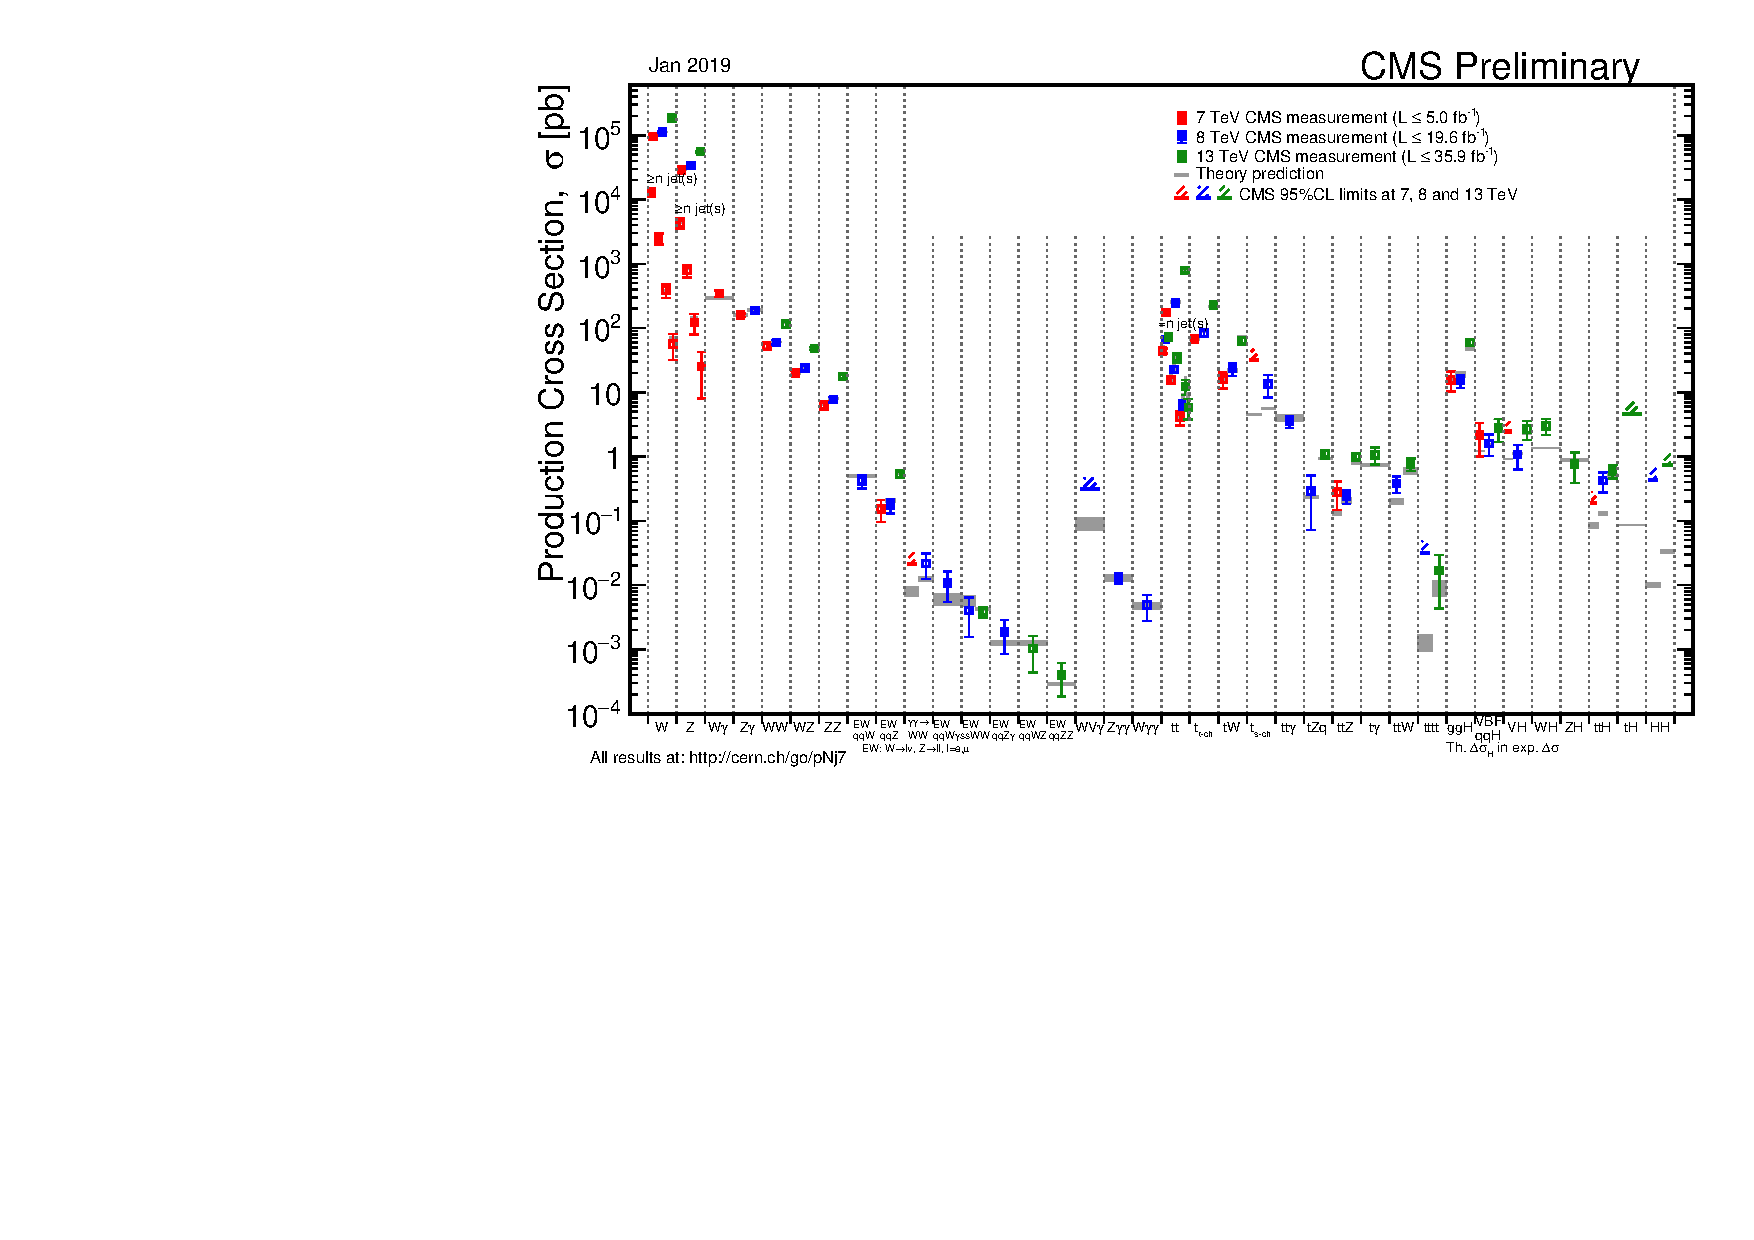
\includegraphics[width=0.9\linewidth]{../Figures/Chap1/SigmaNew_v0}
\caption[SM cross section measurements by CMS]{Summary of the cross section measurements of SM processes by CMS experiment \cite{SMxsec}.}
\label{fig:SigmaNew_v0}
\end{figure*}

Although H was the last piece in the SM puzzle and we have discovered it, there are many theoretical issues and experimental observations
which are not explained by the SM. From the theoretical point of view, observed mass of H at 125 \gev itself is an issue and it is called as 
hierarchy problem which is discussed below. Some of the unsolved problems within SM framework are:
\begin{itemize}
\item The \higgs boson gets corrections to its mass by loop diagram contributions, the largest contribution is coming from top quark loop 
diagram (Fig.\ref{fig:hierarchy_problem_higgs}). This contribution is given by
\begin{equation}
\Delta m_{H}^2 = -\frac{|\lambda_t|^2}{8\pi^2}[\Lambda_{UV}^2 + \dots]
\label{eqn:HmassCorr}
\end{equation}
where $\lambda_t$ is the top Yukawa coupling ($\sim 1$) and $\Lambda_{UV}$ is the ultraviolet cutoff scale above which SM is not valid and 
its value is close to the GUT (grand unified theory) scale \footnote{the scale at which the strength of EM, strong and weak force merge.}, 
$10^{16}\ \gev$ or Planck scale, $> 10^{19}\ \gev$. With these large corrections, the mass of \higgs would have been $> 10^{16}\ \gev$ and 
not near 125 \gev. This is called hierarchy problem in SM. It is very \textit{unnatural} to have a contribution $\sim 10^{16}$ \gev which 
cancels the effect shown in eqn.\ref{eqn:HmassCorr} and get mass of Higgs as 125 \gev.
\begin{figure}[h!]
\centering
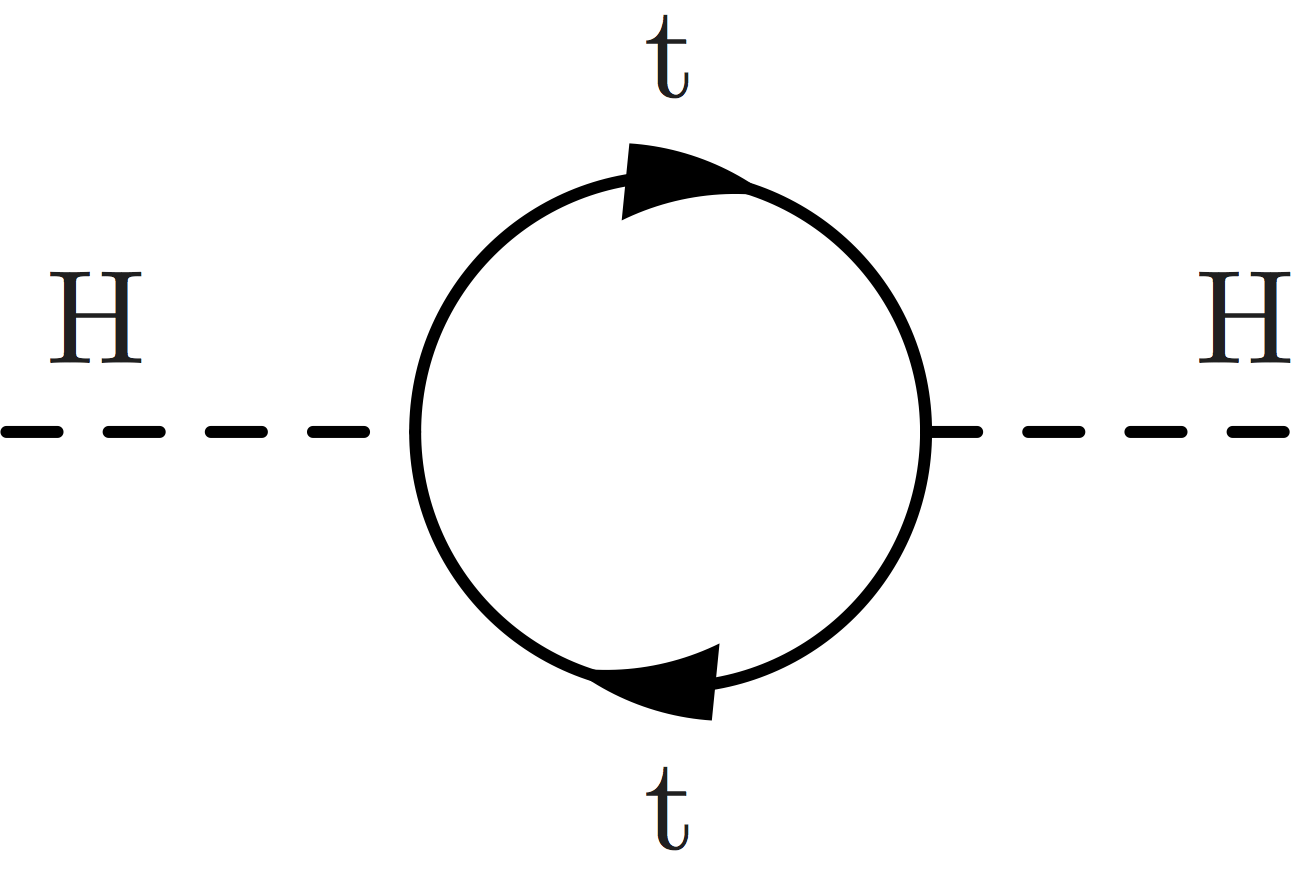
\includegraphics[width=0.35\linewidth]{../Figures/Chap1/hierarchy_problem_higgs.png}
\caption{Top loop diagram contribution to \higgs mass}
\label{fig:hierarchy_problem_higgs}
\end{figure}
\item Gravitational interactions cannot be explained by the SM.
\item Matter-antimatter asymmetry: We do not understand why we see more matter in the universe than antimatter today. At the early stages 
of universe, both of these must have been created in equal amount. There must be a mechanism by which matter started to dominate over 
antimatter.
\item In SM masses of neutrinos is zero, whereas neutrino oscillations \cite{Fukuda:1998mi} indicate that they have nonzero mass.
\item The universe comprises of 71.4\% of dark energy, 24\% of dark matter and only 4.6\% is ordinary matter that we know. What is 
explained by SM is less than 5\% of the total universe content.
\item The strong, EM and weak gauge couplings are functions of energy scale. When these couplings are extrapolated to high energy, we 
expect all of them to unify at one energy. But this unification does not take place at one point within SM.
\end{itemize}

\section{Supersymmetric extension of the SM}
To overcome the limitations of the SM mentioned in Sec.\ref{SMLimitations}, we need extensions to SM which can address all (or some) of these 
issues without contradicting existing observations. One such extension is supersymmetry (SUSY) which can address some of the issues 
mentioned above, namely the dark matter problem, gauge coupling unification and hierarchy problem.

To tackle hierarchy problem, if we can introduce a new term in eqn.\ref{eqn:HmassCorr} with similar correction but opposite sign, we might 
be able to get \higgs mass around 125 \gev. Naively speaking, what SUSY does is exactly this - it introduces a scalar partner for every SM 
fermion and a fermionic partner for every bosonic SM particle and hence the corrections from superpartner loop diagrams cancel the 
corrections from SM particle loop diagrams. 
Superpartners of SM particles differ in spin by half a unit. For example, superpartner of top quark is top 
\textbf{s}quark (or \textbf{s}top) with spin 0. The superpartners of bosons have spin \textonehalf\ and they are named with suffix 
\textit{ino}, such as gluino, photino etc. Fig.\ref{fig:hierarchy_problem_higgs_mass_stop} shows the contributions to \higgs mass from top 
loop and stop loop. The contribution from second loop diagram is given by eqn.\ref{eqn:HmassCorrSUSY} which has similar form as 
eqn.\ref{eqn:HmassCorr} but with an opposite sign.
\begin{figure*}[h!]
\centering
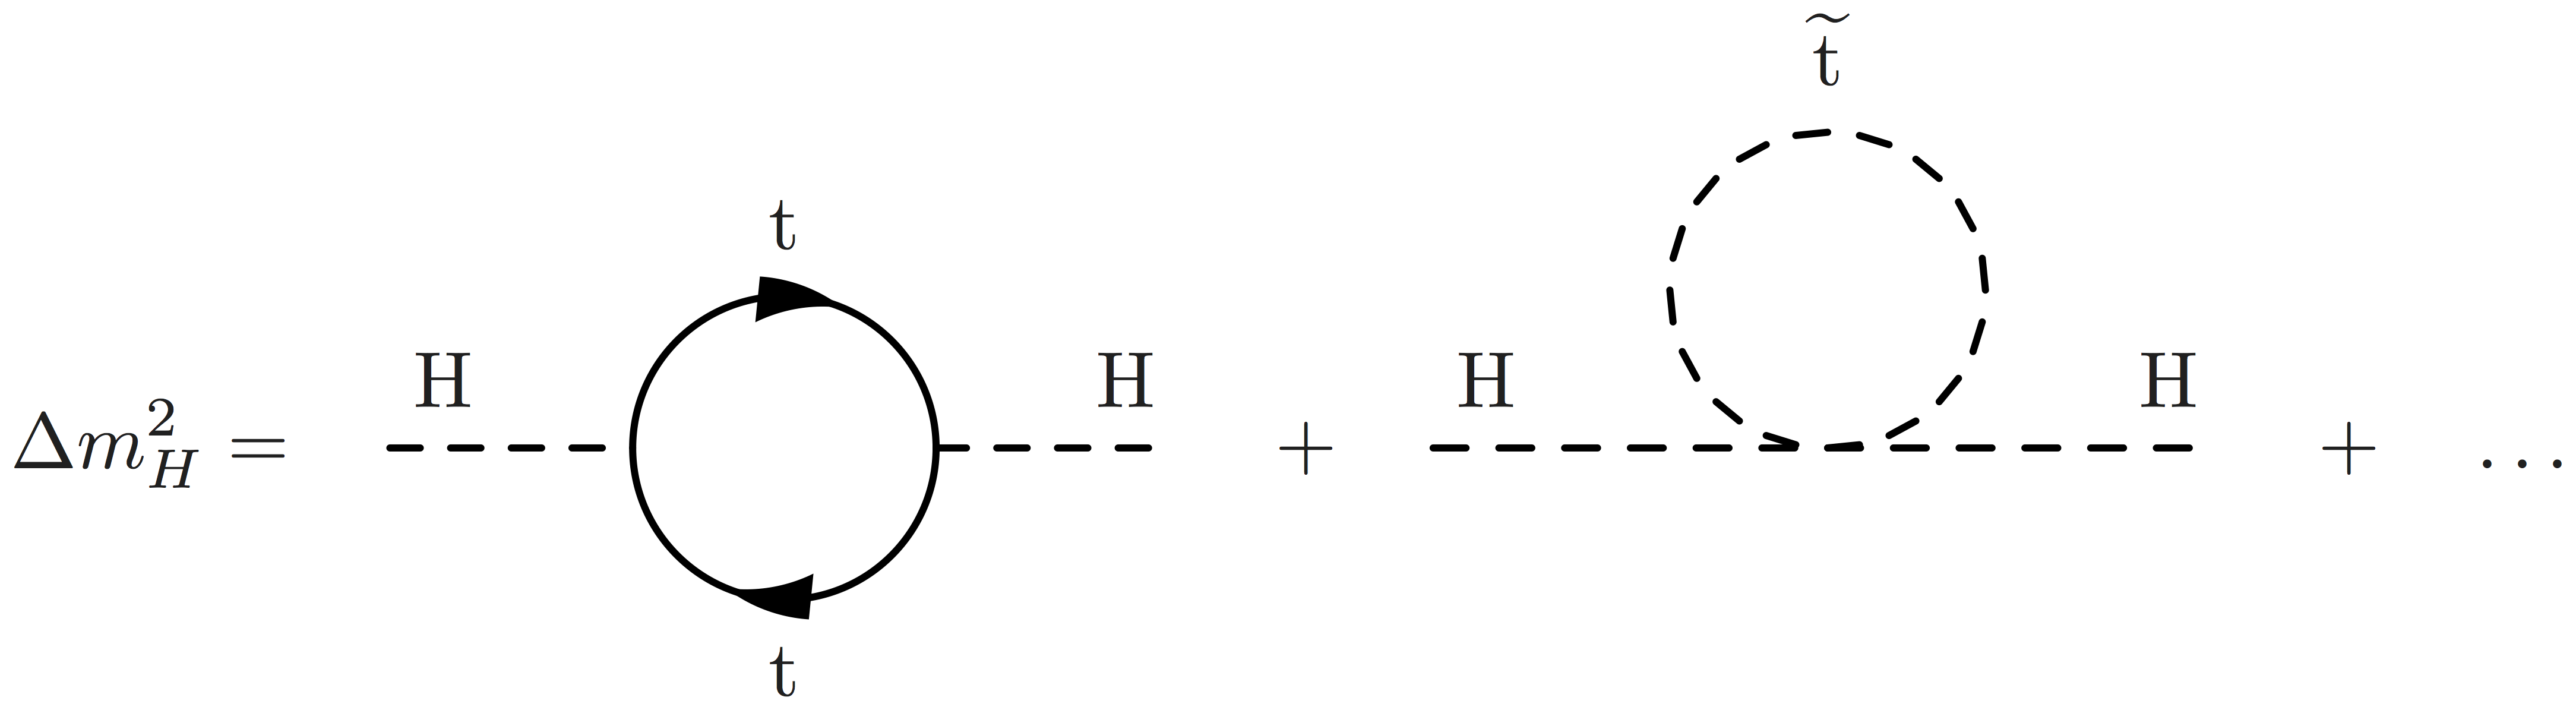
\includegraphics[width=0.8\linewidth]{../Figures/Chap1/hierarchy_problem_higgs_mass_stop}
\caption{Corrections to \higgs mass from top loop and stop loop.}
\label{fig:hierarchy_problem_higgs_mass_stop}
\end{figure*}
\begin{equation}
(\Delta m_{H}^2)_{\text{SUSY}} = \frac{|\lambda_{\tilde{t}}|^2}{8\pi^2}[\Lambda_{UV}^2 + \dots]
\label{eqn:HmassCorrSUSY}
\end{equation}

We are interested in minimal supersymmetric extension of SM (MSSM) which is direct supersymmetrization of SM and has minimum number of new 
particle states and interactions consistent with phenomenology \cite{baer_tata_2006}. Table \ref{tab:SUSY} shows fields corresponding to 
various particles in the MSSM. These superpartners listed are not necessarily the mass eigenstates of the theory because there can be 
mixing of gauginos and higgsinos \cite{Martin:1997ns}. The observable mass eigenstates are charginos or neutralinos, denoted by 
$\tilde{\chi}^{\pm,\ 0}$ and gluino which is not a mixture. Gauge and mass eigenstates in MSSM are listed in table \ref{tab:SUSY2}.

\begin{table}[h!]
\centering
\caption[Chiral and gauge supermultiplets of MSSM]{Chiral supermultiplets and gauge supermultiplets in the MSSM \cite{Martin:1997ns}}
\label{tab:SUSY}
\begin{tabular}{|c|c|c|}
\hline   & spin 0  & spin \textonehalf  \\ 
\hline  
\multirow{3}{*}{squarks, quarks (x3 families)} & \topMargin$\left(\tilde{u}_L\ \tilde{d}_L \right)$  & (${u_L}\ {d_L}$) \\ 
								               & $\tilde{u}_R$				& $u_R$\\
                      						   & $\tilde{d}_R$				& $d_R$\\ \hline
\multirow{2}{*}{sleptons, leptons (x3 families)} & ($\tilde{\nu}\ \tilde{e}_L$) & (${\nu}\ {e_L}$) \\ 
                      						   & $\tilde{e}_R$				& $e_R$\\ \hline
\multirow{2}{*}{Higgs, higgsinos}			   & \topMargin$(H^{+}_u\ H^{0}_u)$       & $(\tilde{H}^{+}_u\ \tilde{H}^{0}_u)$\\
											   & $(H^{0}_d\ H^{-}_d)$       & $(\tilde{H}^{0}_d\ \tilde{H}^{-}_d)$\botMargin\\ \hline
                      						   & spin \textonehalf					& spin 1 \\ \hline
                  		gluino, gluon		   & $\tilde{g}$				& $g$ \\
                  		winos, W bosons		   & $\tilde{W}^\pm\ \tilde{W}^0$ & $W^\pm\ W^0$ \\
                  		bino, B boson		   & $\tilde{B}^0$				& $B^0$\\ \hline
\end{tabular} 
\end{table}

\begin{table}[h!]
\centering
\caption[Gauge and mass eigenstates of MSSM]{Gauge and mass eigenstates of MSSM \cite{Martin:1997ns}\cite{Rizzi:2646377}}
\label{tab:SUSY2}
\begin{tabular}{c|c|c|c}
\hline
Names	 					&	Spin			&	Gauge eigenstates				&	Mass eigenstates \\\hline
\multirow{3}{*}{squarks}	& \multirow{3}{*}{0}&	\topMargin\susyP{u}$_L$ \susyP{u}$_R$ \susyP{d}$_L$ \susyP{d}$_R$ & same \\
							&					&	\susyP{c}$_L$ \susyP{c}$_R$ \susyP{s}$_L$ \susyP{s}$_R$ & same \\
							&					&	\susyP{t}$_L$ \susyP{t}$_R$ \susyP{b}$_L$ \susyP{b}$_R$ & \susyP{t}$_1$ \susyP{t}$_2$ \susyP{b}$_1$ \susyP{b}$_2$ \\\hline
\multirow{3}{*}{sleptons}	& \multirow{3}{*}{0}&	\susyP{e}$_L$ \susyP{e}$_R$ \susyP{\nu}$_e$ 			 & same \\
							&					&	\susyP{\mu}$_L$ \susyP{\mu}$_R$ \susyP{\nu}$_\mu$		 & same \\
							&					&	\susyP{\tau}$_L$ \susyP{\tau}$_R$ \susyP{\nu}$_\tau$	 &\susyP{\tau}$_1$ \susyP{\tau}$_2$ \susyP{\nu}$_\tau$ \\\hline
\topMargin neutralinos & \textonehalf & \susyP{B}$^0$ \susyP{W}$^0$ \susyP{H}$^{0}_{u}$ \susyP{H}$^{0}_{d}$ & \susyP{\chi}$^{0}_1$ \susyP{\chi}$^{0}_2$ \susyP{\chi}$^{0}_3$ \susyP{\chi}$^{0}_4$ \\\hline
\topMargin charginos & \textonehalf & \susyP{W}$^\pm$  \susyP{H}$^{+}_{u}$  \susyP{H}$^{-}_{d}$ & \susyP{\chi}$^{\pm}_1$ \susyP{\chi}$^{\pm}_2$ \\\hline
gluino 						&	\textonehalf				&	\susyP{g}				&	same \\\hline
\topMargin Higgs bosons				&	0				& \susyP{H}$^{0}_{u}$ \susyP{H}$^{0}_{d}$ \susyP{H}$^{+}_{u}$  \susyP{H}$^{-}_{d}$ & $h^0$ \higgs$^0$ $A^0$ $H^\pm$ \\\hline
\topMargin gravitino	&	3/2	&	\grav	& same \\\hline
\end{tabular}
\end{table}

Since we have not observed supersymmetric particles at the same mass SM counterparts, SUSY is a broken symmetry and the masses of 
sparticles are larger than SM partners. The effective Lagrangian can be written as
\begin{equation}
\label{eqn:Lsusy}
\mathcal{L} = \mathcal{L_{\text{SUSY}}} + \mathcal{L_\text{{soft}}}
\end{equation}
The first term on RHS of eqn.\ref{eqn:Lsusy} preserves SUSY and contains gauge and Yukawa interactions. The second term breaks SUSY and 
contains mass terms and coupling parameters which should vanish at very high mass scale at which SUSY is unbroken. There are multiple ways 
to break SUSY and some of the popular ways are, gravity mediated or Planck scale mediated SUSY breaking (PMSB), anomaly mediated SUSY 
braking (AMSB) and gauge mediated SUSY breaking (GMSB). A brief discussion on GMSB is given in section \ref{sec:gmsb} to motivate the 
search for SUSY with photon which is the topic of this thesis.

\subsection{R-parity}
A multiplicative quantum number called \textit{R-parity} is introduced for every particle and sparticle to account for very strong 
experimental bounds on proton lifetime. The proton lifetime is $>10^{33}$ years \cite{PhysRevLett.102.141801} which is larger than the age 
of the universe.
R-parity is defined as
\begin{equation}
\label{eqn:rparity}
P_R = (-1)^{3(B-L)+2s}
\end{equation}
where s is the spin, B and L are baryon number and lepton number respectively. All SM particles have even R-parity, $P_R=+1$ and 
supersymmetric particles have odd R-parity, $P_R=-1$. If R-parity is not conserved, then $p\to e^+\pi^{0}$ via anti-squark mediation as 
shown in Figure \ref{fig:protonDecay}.
\begin{figure}[h!]
\centering
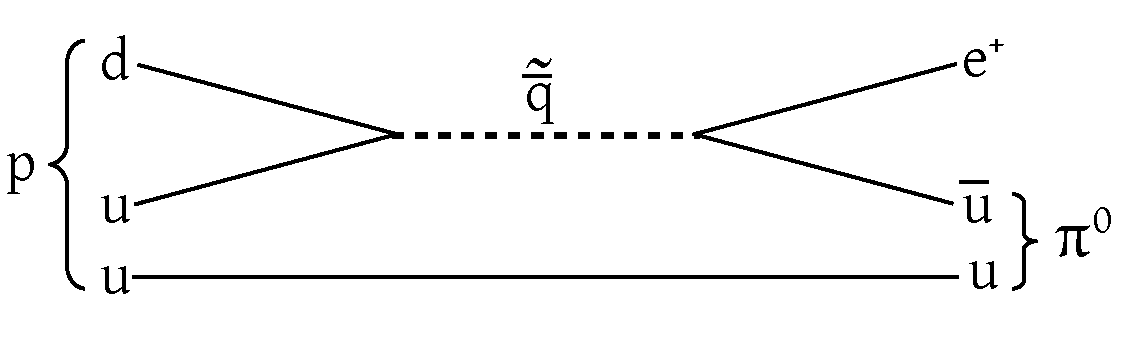
\includegraphics[width=0.7\linewidth]{../Figures/Chap1/protonDecay}
\caption[Proton decay diagram]{One of the possible modes for decay of proton via anti-squark mediation if R-parity is not conserved.}
\label{fig:protonDecay}
\end{figure}

Important consequences \cite{Martin:1997ns} of R-parity conservation are:
\begin{itemize}
\item Supersymmetric particles are always produced in pairs in collider experiments
and any supersymmetric particle decay should involve odd number of daughters.
In other words, at any vertex, there should be even number of supersymmetric particles.
\item Lightest supersymmetric particle (LSP) must be stable. If LSP is neutral and weakly interacting, then it could serve as a dark matter 
candidate and account for 24\% (or some part of 24\%) of the universe content \cite{ELLIS1984453}.
\item All the non-LSP supersymmetric particle decay chains must result in odd number (usually 1) of LSPs.
\end{itemize}

\section{Gauge mediated SUSY breaking}
\label{sec:gmsb}
In GMSB scenarios \cite{Dine:1993yw,Dine:1994vc,Dine:1995ag,Meade:2008wd,Giudice:1998bp,Grajek:2013ola}, the communication between hidden 
sector, where SUSY breaking takes place, and the visible MSSM sector (consisting of chiral supermultiplets shown in table \ref{tab:SUSY2}) 
is via the ordinary gauge interactions. In comparison with other SUSY breaking scenarios, flavor changing processes and new sources of CP 
violation are naturally suppressed \cite{Dine:1993yw} in GMSB. The messengers communicating between MSSM and hidden sector also have 
$SU(3)_C \otimes SU(2)_L \otimes U(1)_Y$ interactions. The soft terms in MSSM come from loop diagrams involving these messengers, whose 
value is given by
\begin{equation}
m_{soft} \sim \frac{\alpha_{a}}{4\pi} \frac{\langle F \rangle}{M_{mess}}
\end{equation}
where $\alpha_{a}/{4\pi}$ is loop factor for Feynman diagrams involving gauge interactions, $F$ relates to the SUSY breaking scale and 
$M_{mess}$ is the messenger mass scale \cite{Martin:1997ns}.

GMSB permits a significantly lower symmetry-breaking scale ($\langle F\rangle$) than, e.g., gravity mediation, and therefore generically 
predicts that the gravitino (\susyP{\mathrm{G}}) is the LSP~\cite{Meade:2008wd,PhysRevLett.38.1433,CREMMER1978231} whose mass is given by
\begin{equation}
\label{massGrav}
m_{\grav}  \sim \ \langle F \rangle/M_P \sim \mathrm{keV}
\end{equation}
where $M_P$ is the Planck scale where gravity is expected to become strong.

\subsection{Phenomenology of GMSB}
As mentioned above, gravitino ($\tilde{\mathrm{G}}$), superpartner of graviton, is the LSP, it is stable and weakly interacting and 
results in missing transverse momentum. The next-to-LSP (NLSP) is either a neutralino ($\susyP{\chi}_{1}^{0}$) or a chargino 
($\susyP{\chi}_{1}^{\pm}$). The decay modes of the NLSP is decided by its nature - bino, wino and higgsino components in it 
\cite{Knapen:2016exe}.
\begin{itemize}
\item For a \textbf{bino like} NLSP, $|M_1| < |\mu|, |M_2|$, where $M_1, M_2$ and $\mu$ are $U(1)$ gauge mass parameter, $SU(2)$ gauge 
mass parameter and higgsino mass parameter respectively. The decay mode of NLSP is $\gamma/Z +$\grav with larger branching ratio (BR) for  
$\gamma +$\grav. The left plot in Fig.\ref{fig:NLSPwinoBinoBR} shows BR for NLSP decay as a function of bino mass \cite{Ruderman:2011vv}.\\
It is worth noting that the coupling of $\gamma$ with \susyP{\mathrm{G}} is at the tree-level because the gravitino has become massive 
after SUSY breaking and it has goldstino component \cite{Martin:1997ns}.\\
Experimentally, these kind of scenarios can be targeted using collider searches with $\gamma\gamma+\ptmiss$ or $\gamma+\ptmiss$ final 
states, where \ptmiss is the magnitude of missing transverse momentum.

\begin{figure*}[h!]
\centering
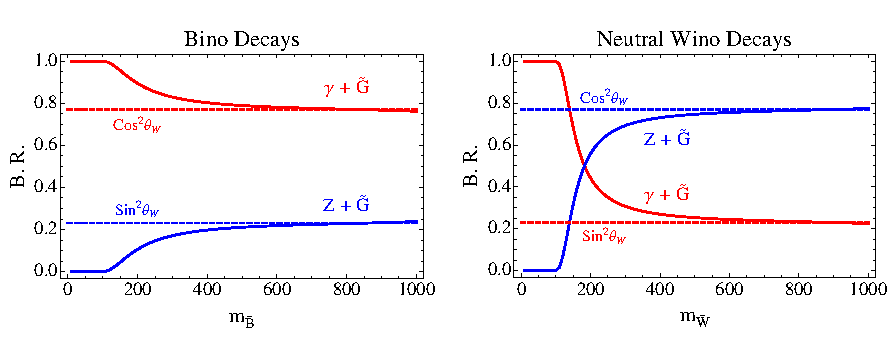
\includegraphics[width=0.8\linewidth]{../Figures/Chap1/NLSPwinoBinoBR}
\caption[BR for bino and neutral wino NLSP decays]{BR for bino and neutral wino NLSP decays. Plot is taken from Ref.\cite{Ruderman:2011vv}}
\label{fig:NLSPwinoBinoBR}
\end{figure*}

\item For a \textbf{wino like} NLSP, $|M_2| < |\mu|, |M_1|$. In this case, \nuone and \chone are nearly mass degenerate and the decay 
modes are
\begin{center}
$\chone \rightarrow W^\pm + $\grav \\%or ($\pi^{\pm} +$ \nuone + $\grav)\\
$\nuone \rightarrow Z/\gamma + $\grav
\end{center}
The right plot in Fig.\ref{fig:NLSPwinoBinoBR} shows BR for \nuone decay as a function of wino mass \cite{Ruderman:2011vv}. These 
scenarios can result in signatures with lepton $+\ \gamma+\ptmiss$.

\item For a \textbf{higgsino like} NLSP, $|\mu| < M_1,M_2$ and different NLSP decay modes are preferred depending on the value of $\mu$.\\
If $\mu < 0$, then $\nuone \rightarrow \higgs/\gamma + $\grav decay is preferred.\\
If $\mu > 0$, then $\nuone \rightarrow Z/\gamma + $\grav decay dominates.\\
Models with higgsino like NLSP may result in $b\bar{b}$, coming from \higgs decay, and $\gamma+\ptmiss$ final states.
\end{itemize}

\subsection{Simplified GMSB models}\label{sec:SMSgmsb}
There are many free parameters in the theory and as a result it is difficult to know the exact experimental signatures.
A realistic SUSY scenario, if exits and accessible at the LHC, would give signature as one or more of the following event topologies - 
0 lepton, 1 lepton, 2 leptons, multiple leptons, at least one photon and 0 lepton, 2 photons and 0 lepton, 1 lepton 
and at least one photon, high \ptmiss, multiple jets etc.
Generally, the searches at CMS are designed based on these final state signatures. Once the final state is decided, certain
assumptions are made on the models and they are called as simplified model scenarios (SMS) 
\cite{bib-sms-1,bib-sms-2,bib-sms-3,bib-sms-4,Chatrchyan:2013sza} which are used to design SUSY searches.

For example, one of the SMS considered in this thesis is shown in Figure \ref{fig:T5bbbbZG_sms}. 
\begin{figure*}[htb]
\centering
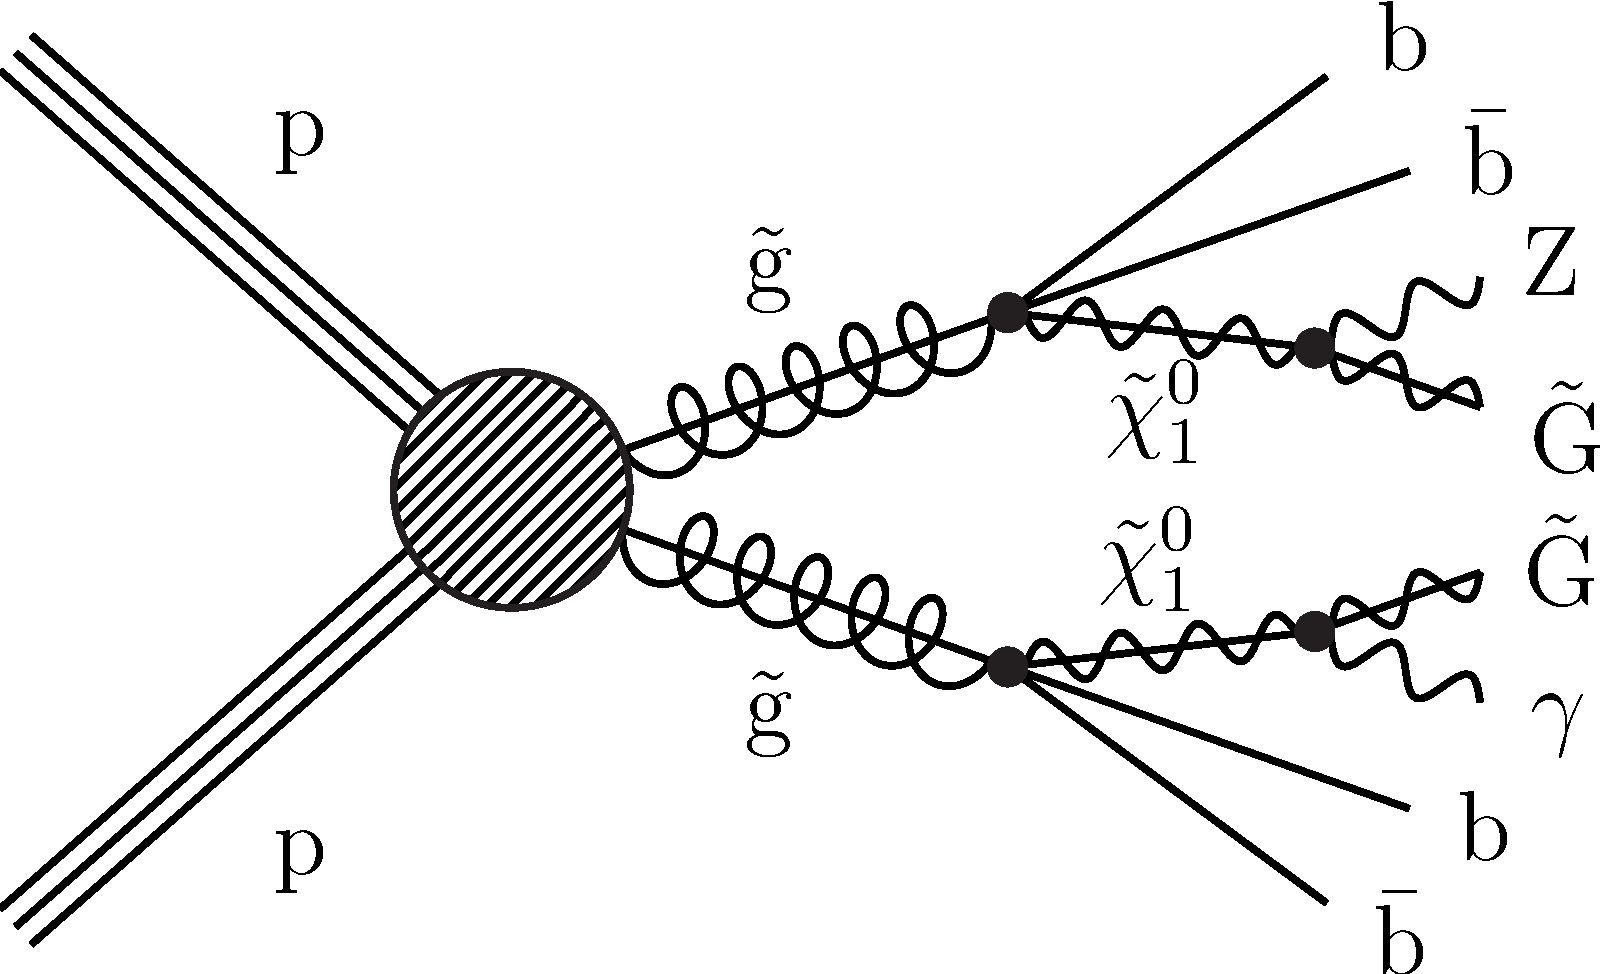
\includegraphics[width=0.4\linewidth]{../Figures/Chap1/Figure_001-b.pdf}\\
\caption[SMS diagrams]{SMS diagram showing decay of gluino to \bbbar\ and \nuone. Then, \nuone decays to \grav and $\gamma$/Z.}
\label{fig:T5bbbbZG_sms}
\end{figure*}
In this case, we have assumed
\begin{itemize}
\item All sparticles, except gluino, \nuone and \grav are very heavy and not accessible at the LHC.
\item Gluino decays to \bbbar\ and \nuone with 100\% branching ratio (BR).
\item \nuone decays to \grav + $\gamma$ or \grav + Z with 50\% BR each.
\end{itemize}
A typical signature of this model is large \ptmiss, many jets and b-jets and photon. A realistic GMSB SUSY model is more complicated
with many free parameters and designing a search is very difficult in those cases. If the GMSB scenario is realized in nature
and gives similar final states as the one shown in Figure \ref{fig:T5bbbbZG_sms}, then this search might be able to discover it.
On the other hand, if the final state is different than what is studied here, other searches would be able to discover it. In this way
it is possible to explore large phase-space easily and increase the chances of discovery.  Another advantage in using SMS 
is that it is easy to re-interpret the results by taking a different SUSY model.